\documentclass{beamer}

\usepackage{color}
\usepackage{ctex}
\usepackage{graphicx}
\usepackage{beamerthemesplit}
\usepackage{caption}
\usepackage{graphicx, subfig}
\usepackage{bm}
\usepackage{mathrsfs}
\usepackage{fontspec}



\title{Diffusion Convolutional Recurrent Neural
Network: Data-Driven Traffic Forecasting}
\author{Zhou Hao}
\date{2018.11}

\begin{document}
 	\frame{\titlepage}
 	\section*{Outline}
 	\frame{\tableofcontents}

  \section{Introduction}
  \frame{
  \textbf{Introduction} \\ 
  Traffic forecasting is challenging:
  \begin{itemize}
    \item complex spatial dependency on road networks
    \item non-linear temporal dynamics with changing road conditions
    \item inherent difficulty of long-term forecasting
  \end{itemize}
  \begin{figure}
  \centering
  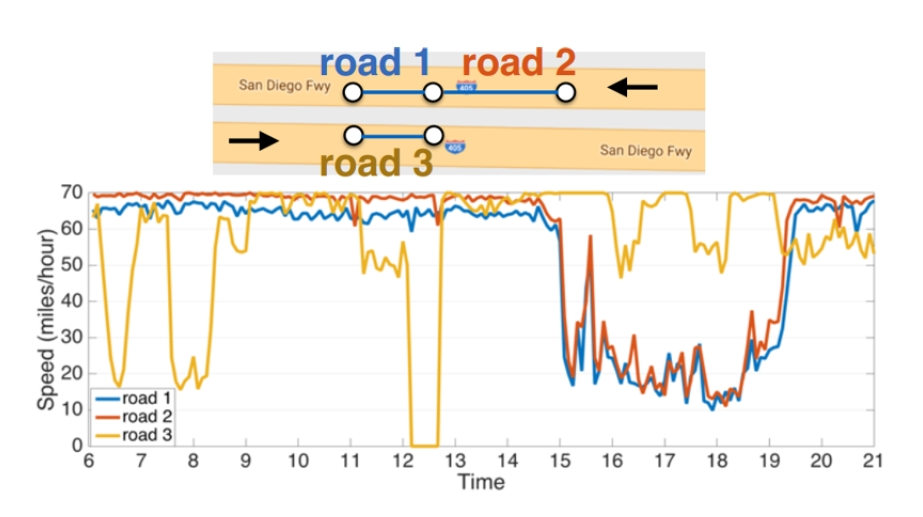
\includegraphics[width=.8\textwidth]{fig1.jpg}
  \end{figure}
  }
  
  \frame{
  In this work:
  \begin{itemize}
      \item Model the spatial dependency of traffic as a diffusion process on a directed graph and Propose \textit{diffusion convolution}
      \item Propose \textit{Diffusion Convolutional Recurrent Neural Network} (DCRNN)
      \item Conduct experiments on two large-scale real-world datasets and obtain significant improvement
  \end{itemize}
  }
  
  \section{Methodology}
  \subsection{Traffic forecasting Problem}
  \frame{
  The goal of traffic forecasting is to predict the future traffic speed given previously observed traffic flow from $N$ correlated sensors on the road network.
  
  $$[\bm{X}^{(t-T'+1)},\dots,\bm{X}^{(t)};\mathscr{G}] \xrightarrow{h(\cdot)} [\bm{X}^{(t+1)},\dots,\bm{X}^{(t+T)}]$$
  }
  
  \subsection{Spatial Dependency Modeling}
  \frame{
  \begin{itemize}
      \item This diffusion process is characterized by a random walk on $\mathscr{G}$ with restart probability $\alpha \in [0,1]$
      \item state transition matrix $\bm{D}_O^{-1}\bm{W}$
      \item $\bm{D}_O = \text{diag}(\bm{W1})$
      \item after many time steps, such Markov process converges to a stationary distribution $\bm{P} \in \mathbb{R}^{N \times N}$
      \item $$\bm{P} = \sum_{k=0}^{\infty} \alpha (1-\alpha)^k(\bm{D}_O^{-1}\bm{W})^k$$
  \end{itemize}
  }
  
  \frame{
  \textbf{Diffusion Convolution} \\
  The resulted diffusion convolution operation over a graph signal $\bm{X} \in \mathbb{R}^{N \times P}$ and a filter $f_{\theta}$ is defined as:
  \begin{figure}
  \centering
  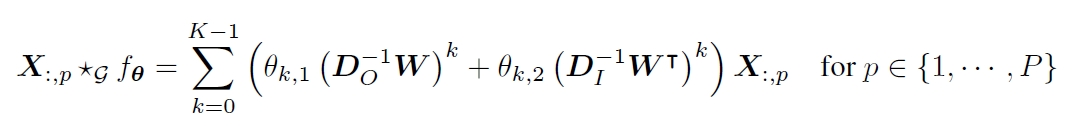
\includegraphics[width=1\textwidth]{fig2.jpg}
  \end{figure}
  \begin{itemize}
      \item $\bm{\theta} \in \mathbb{R}^{K \times 2}$ are the parameters for the filter
      \item $\bm{D}_O^{-1}\bm{W}$,$\bm{D}_I^{-1}\bm{W}^{\intercal}$ represent the transition matrices of the diffusion process and the reverse one.
  \end{itemize}
  }
  
  \frame{
  \textbf{Diffusion Convolutional Layer}\\
  With the convolution operation defined, we can build a diffusion convolutional layer that maps P-dimensional features to Q-dimensional outputs.\\
  Denote the parameter tensor as $\Theta \in \mathbb{R}^{Q \times P \times K \times 2} = [\theta]_{q,p}$, where $\Theta_{q,p,:,:} \in \mathbb{R}^{K \times 2}$ parameterizes the convolutional filter for the $p$th input and the $q$th output.
  
  \begin{figure}
  \centering
  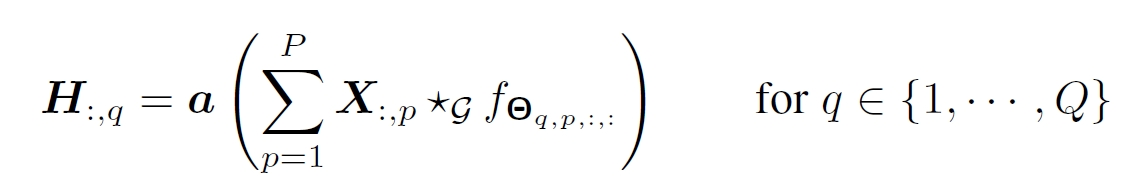
\includegraphics[width=1\textwidth]{fig3.jpg}
  \end{figure} \\
  $a$ is the activation function }
  
  \subsection{Temporal Dynamics Modeling}
  \frame{
  \textbf{Gated Recurrent Units (GRU)}\\
  \begin{itemize}
      \item a simple yet powerful variant of RNNs
      \item replace the matrix multiplications in GRU with the \textit{diffusion convolution}
      \begin{figure}
      \centering
      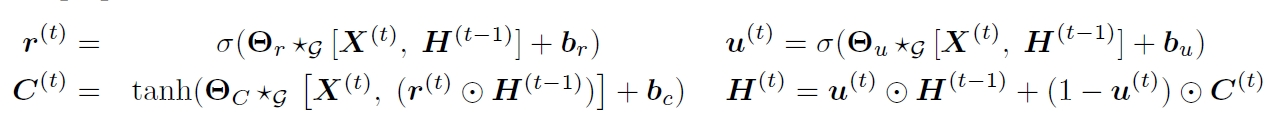
\includegraphics[width=.8\textwidth]{fig4.jpg}
      \end{figure}
      \item DCGRU can be used to build recurrent neural network layers and can be trained using backpropagation through time
  \end{itemize}
  }
  
  \frame{
  \textbf{Sequence to Sequence architecture}\\
  \begin{figure}
  \centering
  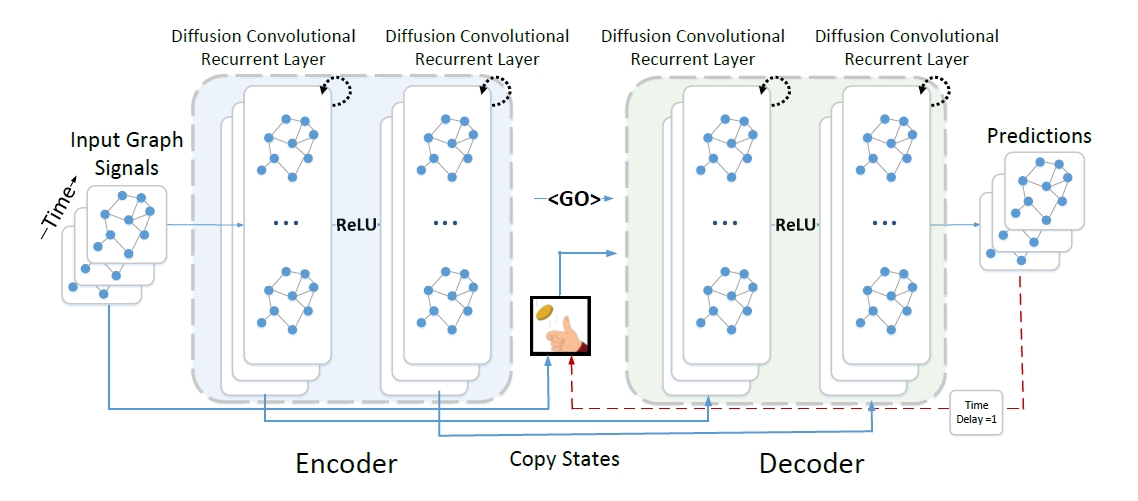
\includegraphics[width=.8\textwidth]{fig5.jpg}
  \end{figure} \\
  }
  
  \frame{
  \begin{itemize}
      \item both the encoder and the decoder are recurrent neural networks with DCGRU
      \item feed the historical time series into the encoder and use its final states to initialize the decoder
      \item \textit{scheduled sampling}\\
      The decoder makes predictions based on either previous ground truth or the model output
  \end{itemize}
  }
  
  \section{Experiments}
  \subsection{Traffic Forecasting Performance Comparison}
  \frame{
  \textbf{two real-world large scale datasets:}
  \begin{itemize}
      \item \textbf{METR-LA}\\
      traffic information collected from loop detectors in the highway of Los Angeles County
      \item \textbf{PEMS-BAY}\\
      traffic dataset collected by California
Transportation Agencies (CalTrans) Performance Measurement System (PeMS)
  \end{itemize}
  }
  
  \frame{
  \begin{figure}
  \centering
  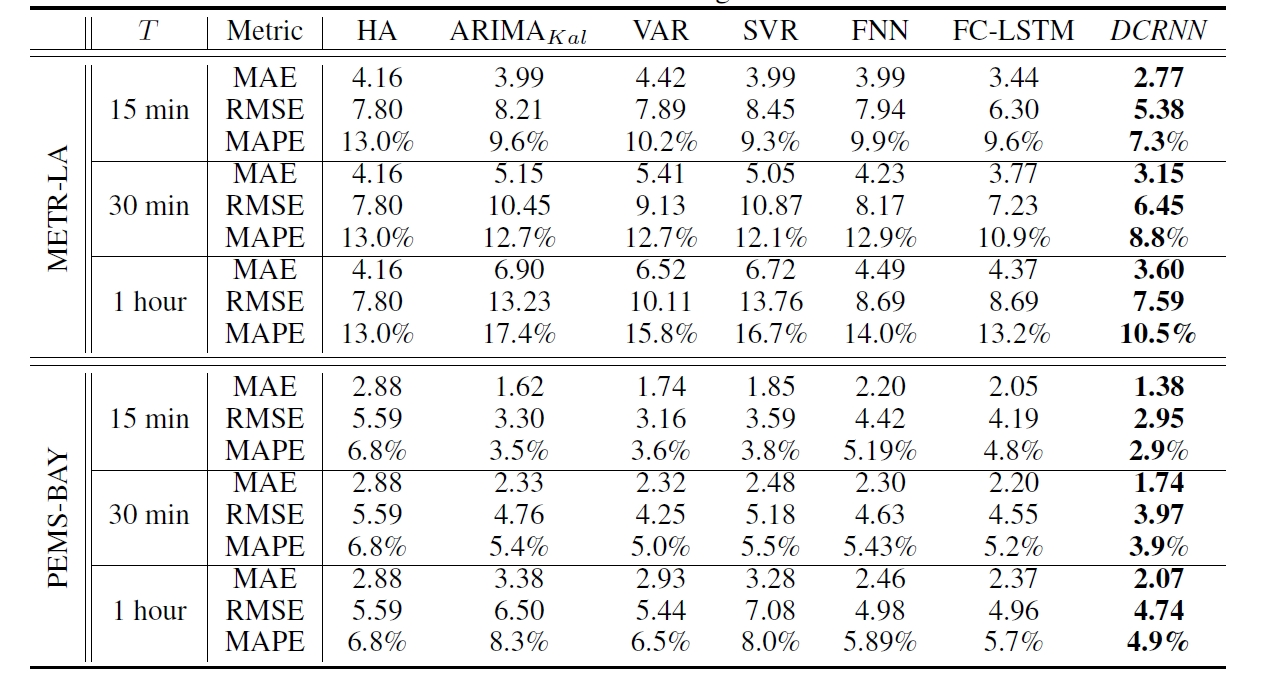
\includegraphics[width=1\textwidth]{fig6.jpg}
  \end{figure}
  }
  
  \frame{
  We observe the following phenomenon in both of these datasets:
  \begin{itemize}
      \item RNN-based methods, including FC-LSTM and DCRNN, generally outperform other baselines which emphasizes the importance of modeling the temporal dependency.
      \item DCRNN achieves the best performance regarding all the metrics for all forecasting horizons
      \item Deep neural network based methods including FNN, FC-LSTM and DCRNN, tend to have better performance than linear baselines for long-term forecasting, e.g., 1 hour ahead
  \end{itemize}
  }
  
  \subsection{Effect of Spatial Dependency Modeling}
  \frame{
  \begin{itemize}
      \item DCRNN-NoConv, which ignores spatial dependency by replacing the transition matrices in the diffusion convolution with identity matrices. This essentially means the forecasting of a sensor can be only be inferred from its own historical readings;
      \item DCRNN-UniConv, which only uses the forward random walk transition matrix for diffusion convolution
  \end{itemize}
  \begin{figure}
  \centering
  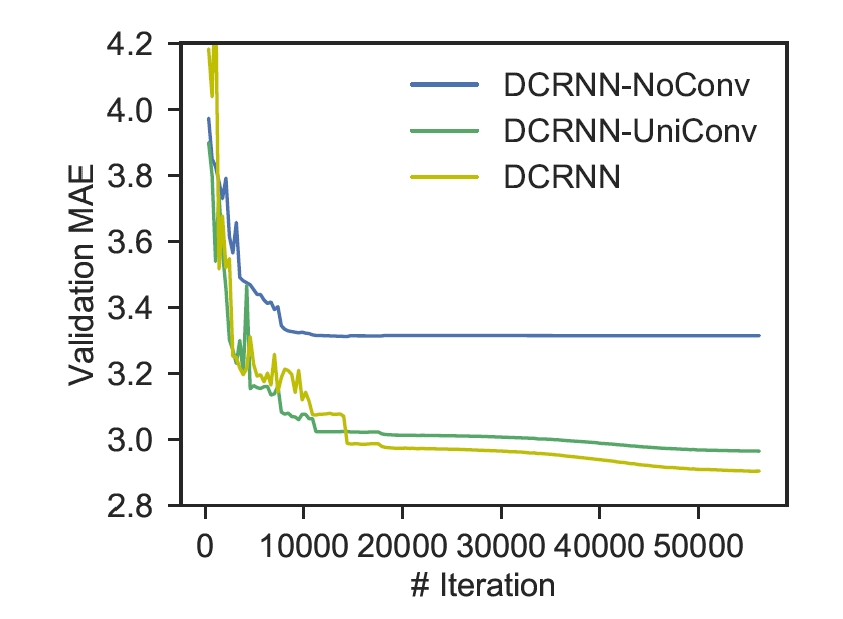
\includegraphics[width=.5\textwidth]{fig7.jpg}
  \end{figure}
  }
  
  \subsection{Effect of Temporal Dependency Modeling}
  \frame{
  \begin{itemize}
      \item DCNN: We train a single model for one step ahead prediction, and feed the previous prediction into the model as input to perform multiple steps ahead prediction.
      \item DCRNN-SEQ: uses the encoder-decoder sequence to sequence learning framework to perform multiple steps ahead forecasting.
      \item DCRNN: similar to DCRNN-SEQ except for adding scheduled sampling
  \end{itemize}
  \begin{figure}
  \centering
  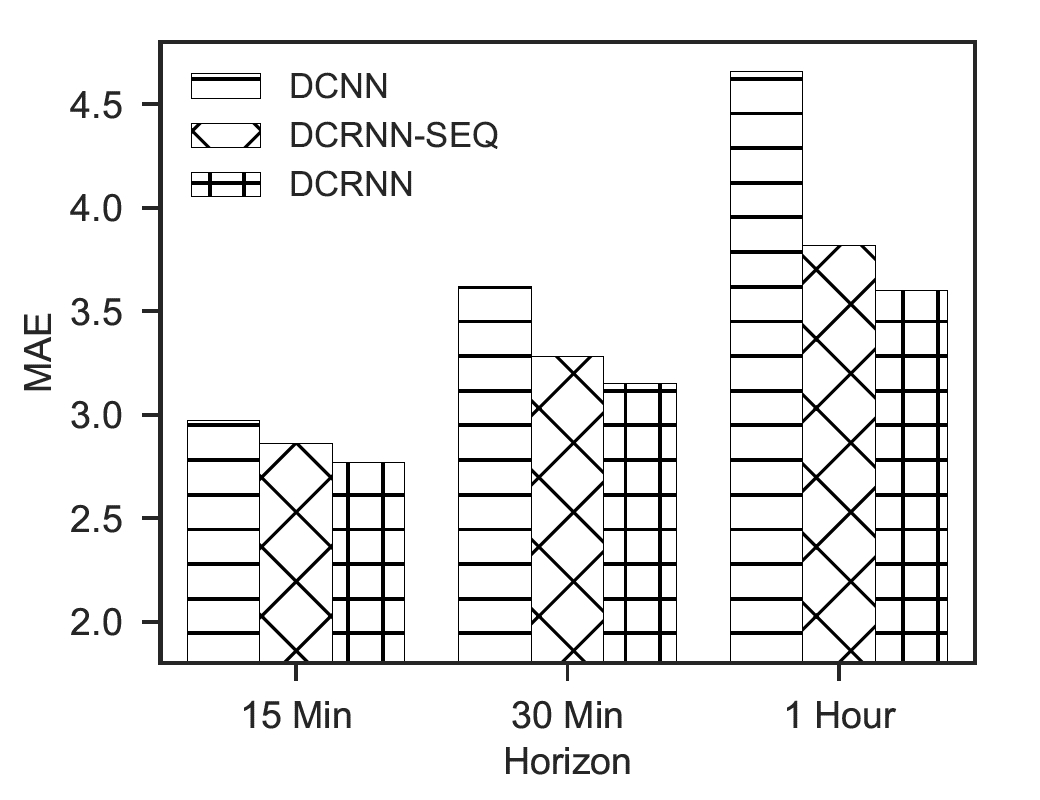
\includegraphics[width=.5\textwidth]{fig8.jpg}
  \end{figure}
  }
  
  \subsection{Model Interpretation}
  \frame{
  \begin{figure}
  \centering
  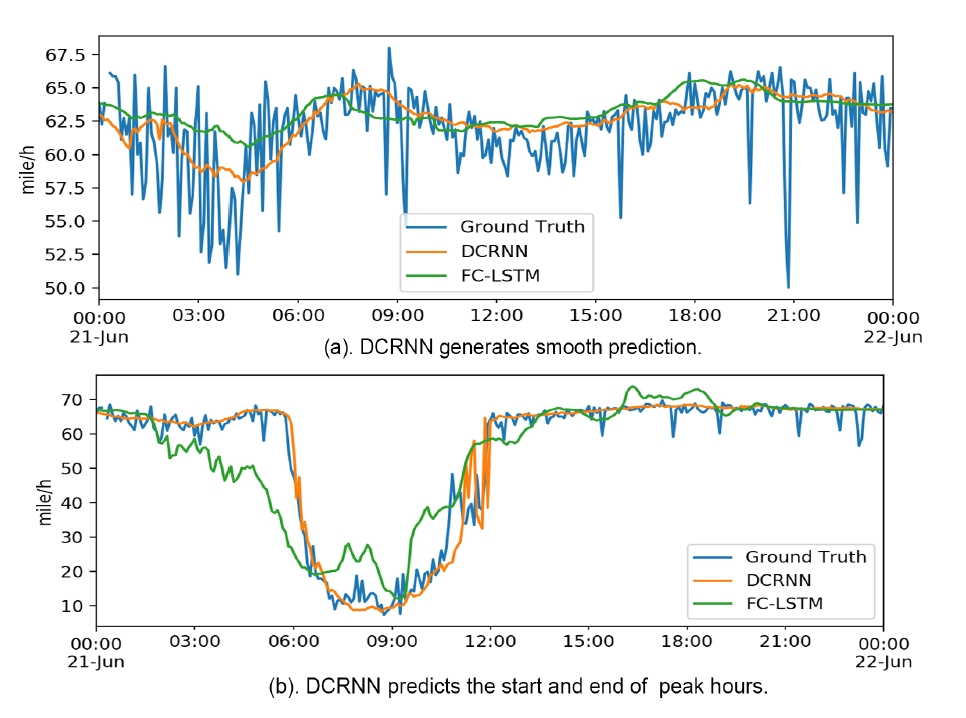
\includegraphics[width=.9\textwidth]{fig9.jpg}
  \end{figure}
  }
 
\end{document}
